\section{Problem Definition} \label{sec:prob}
In this section, we first describe the related background, i.e., page allocation and deallocation in guest OS, page table security validations, and the DMA security validations.
Then, we highlight the identified two performance issues: 1) long execution paths of the guest page table (de)allocation and 2) the additional IOTLB flushes.
As Xen~\cite{XEN-SOSP03} is a typical and popular paravirtual hypervisor, we use Xen in a x86 MMU model~\cite{x86-pv-model} to illustrate the details. 
The presented or similar mechanisms would be available on other paravirtual setting.
 
\subsection{Page Allocation and Deallocation}
To allocate a page, the guest kernel has to invoke the system allocators, typically from slab allocator to buddy allocator.
The slab allocator consists of a variable number of caches that are linked together on a doubly linked circular list. 
Each cache maintains blocks of contiguous pages in memory called slabs, which are carved up into small chunks for the data structures and objects. 
When \emph{kmalloc} is called, all it does is searching through the prepared caches. 
If there is no suitable object, the buddy allocator will be involved.
The Buddy allocator manages all free pages that are allocated in blocks with the sizes of powers of 2.  
When the allocation function is invoked, it first searches for blocks of pages of the size requested following the chain.
If no blocks of the requested size are free, blocks of the next size (which is twice that of the size requested) are looked for. 
This process continues until all of the free area has been searched or until a block of pages has been found. 

In contrast to the page allocation, the page deallocation is to return the page back to the system.
The deallocation process may also invoke slab allocator and/or buddy allocator, and would trigger the updates of the corresponding data structures, 
e.g., the buddy allocator always attempts to recombine the freed pages into larger blocks.

In brief, the page allocation and deallocation are time costly due to the deep invocations and complex updates of the dependent data structures.


\subsection{Page Table Validations}\label{sec:pv-security}

Page tables are used by a hardware, i.e., Memory Management Unit (MMU), to translate the linear addresses into physical addresses used by the hardware to execute instructions.
In the PAE-enabled paging mode, a page table has three levels: L1 level (bottom level), L2 level (middle level) and L3 level (top level).
The slots in L1, L2 and L3 levels are known as Page Table Entry (PTE), Page Middle Directory (PMD) and Page Global Directory (PGD), respectively.
A PTE slot could determine the access permissions of a page, e.g., the kernel could set a page as read-only by clearing the bit within a PTE slot that represents the writable permission.
There are many page tables in a guest VM, as each user process has its own page tables.
The creation and exit of a user process will be accompanied by the creation and destruction of a page table respectively.
%It means that if there are numerous temporary processes generated within a period, there will be a large number of page tables created.

In order to ensure that the guest cannot subvert the system, Xen requires that certain update policies are maintained,
and thus all updates of the page tables should be vetted by Xen.
To this end, the guest OS is deprivileged, from ring-0 to ring-1, leaving ring-0 for the Xen hypervisor.
This prevents the guest OS from executing privileged instructions, e.g., the guest OS cannot directly update control registers.

Xen also defines a number of page types, which are listed in Table~\ref{tab:pagetype}, and maintain a type reference count for each page.
Xen enforces the policies that any given page has exactly one type at any given time,
and only pages with the writable type have a writable mapping in the page tables.
By doing this it can ensure that the guest OS is not able to directly modify any page-table pages and therefore subvert the security of the whole system.
If the guest kernel attempts to update the page table, it has to issue a hypercall to ask the hypervisor to complete the update.
As Xen is always involved in all updates of the page tables, the policies on the page table updates are non-bypassable.

Whenever a page table is loaded into the hardware page-table base register (cr3),
the hypervisor takes an appropriate type reference with the L3 page-table type.
If the page is not already of the required type, then in order to take the initial reference it must first have a type count of zero.
In addition, it must be validated to ensure that it follows the following policy:
for a page with a page-table type to be valid, it is required that any pages referenced
by a present page table entry in the page have the type of the next level down.
For instance, any page referenced by a page with type L3 Page Table must itself have the type L2 Page Table.
This policy is applied recursively down to the L1 page table layer.
At L1 the invariant is that any data page mapped by a writable page table entry must have the writable page type.
By applying these policies, Xen ensures that all page-table pages as a whole are safe to be loaded into the cr3.
Similar requirements are also placed on other special page types, e.g., GTD/LDT pages.

The page type is allowed to be changed.
Xen enforces that the type of a page can only be changed when the type count is zero.
In addition, Xen also requires that every page type update only occur between writable and non-writable pages, as summarized in Figure~\ref{fig:page-type-updates}.

\begin{figure}[ht]
\centering
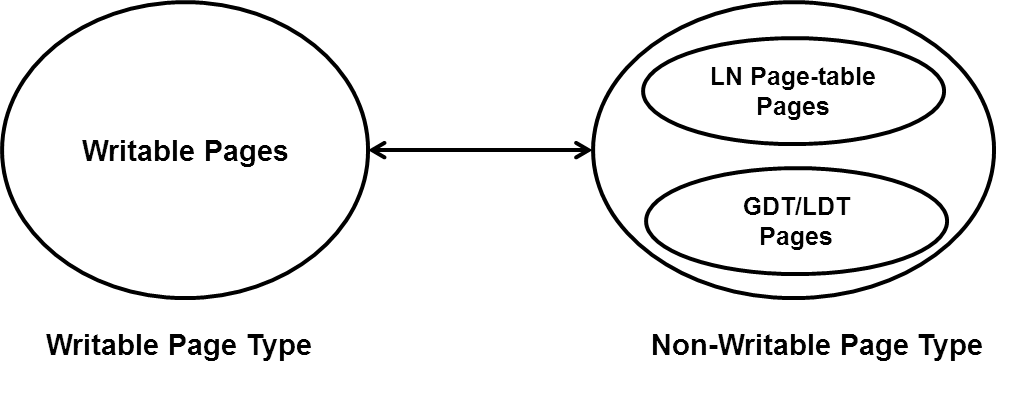
\includegraphics[width=0.45\textwidth]{image/background/page-type-updates.png} \\
\caption{Page Type Updates between writable pages and non-writable pages. (Writable pages are writable for both software and DMA
while non-writable pages are inaccessible to them.)}
\label{fig:page-type-updates}
\end{figure}


\subsection{DMA Validations}

\subsubsection{DMA Address Translation}
%citing: intel vt-d
The input/output memory management unit (IOMMU)~\cite{directio} is a memory management unit (MMU) that connects a DMA-capable I/O bus to the main memory.
Like a traditional MMU, the IOMMU maps device addresses (also called as I/O addresses) to physical addresses through a dedicated page table.
This technique is also known as DMA remapping.
The IOMMU page table that is created and maintained by the hypervisor in its own space, is able to restrict the access on a particular page by configuring the permission bits.
The hypervisor grants different access permissions for different page types, such as the writable pages are always allowed full access permissions, while the page-table pages are always inaccessible to any devices.
This is why when the page-type changes between writable page and page-table page, updating IOMMU page table is always necessary.

However, the DMA remapping always needs the page table walking, which is slow and inefficient.
To accelerate the translation speed, the I/O translation look-aside buffer (IOTLB) is introduced.
The IOTLB is used to cache frequently accessed page table entries.
By doing so, the IOTLB is very likely to be accessed, indicating that the physical address of a queried DMA address will be immediately fetched through the IOTLB path (Figure~\ref{fig:subfig:a}).
If unlikely the IOTLB miss occurs, the DMA remapping still can go the slow page-table path to get the physical address (Figure~\ref{fig:subfig:b}).
To achieve a better I/O performance, the DMA remapping should avoid taking the page-table path as far as possible.

\subsubsection{Negative Impacts}

\begin{figure}[!t]
    \begin{subfigure}{0.5\textwidth}
        
\includegraphics[width=1\textwidth]{image/background/DMA-IOTLB-translation.png}
        \caption{\centering IOTLB Path.}
        \label{fig:subfig:a}
    \end{subfigure}%
    \vfill \vfill \vfill \vfill
    \begin{subfigure}{0.5\textwidth}
        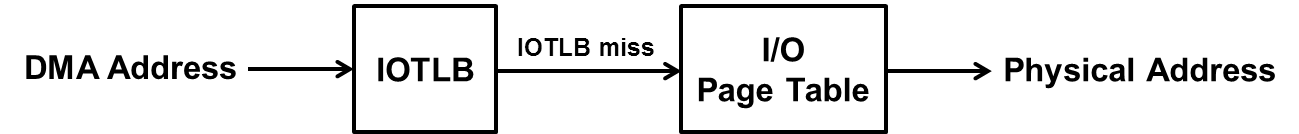
\includegraphics[width=1\textwidth]{image/background/DMA-pt-translation.png}
        \caption{\centering I/O Page-Table Path.}
        \label{fig:subfig:b}
    \end{subfigure}
    \caption{IOTLB path is orders of magnitudes faster than I/O Page-Table Path.}
    \label{fig:dma-add-trans}
\end{figure}


\subsection{Long Execution Path}\label{sec:longpath}
The long execution path issue refers to the execution paths for installing/uninstalling a the guest page table page.
In the current design, installing/uninstalling a page table page has to invoke the complex memory allocators and performance both software (i.e., page table) and DMA validations.
%In addition, the DMA validations always lead to additional IOTLB flushes, which would reduce the DMA address translation speed and may consequently lower the I/O performances.
In addition, such installation and uninstallation events are frequently happened in the system, e.g., the process creation and exits will result in many page-table page installations/uninstallations.
Thus, it is necessary to shorten the execution paths to save CPU usage, benefiting 

%As the uninstallation process of the guest page table page is the reverse to the installation process. In this section, we only present the details of installation.
\subsection{Additional IOTLB Flush Issue}
The dependency between the guest page table and the IOTLB is very subtle.
To fully understand the dependency, we need to know the details about how the paravirtualized hypervisor protects itself through guest page table and IOMMU.
Specifically, we explicitly describe 1) paravirtualized MMU mode, and 2) IOMMU and DMA address translation.

Based on the observations and deep analysis, we know that there are seven page types, and the updates among them always trigger additional IOTLB flushes.
In particular, segment descriptor pages are rarely updated, as they are treated as almost const structures.
However, the page-table pages are frequently updated from/to writable pages.
These updates that are driven by the process creations and exits are frequently triggered in the whole life cycle of a running system.
Thus, they are becoming the main source for contributing the additional IOTLB flushing.

The additional IOTLB flushes are likely to let the DMA address
translations take the slow and inefficient page-table path,
instead of taking the fast and efficient IOTLB path (Figure~\ref{fig:dma-add-trans}), which inevitably lowers the
speed of the whole DMA transfering, especially for the high performance devices.


In brief, we summarize all these into three key points, which are listed as follows:
\begin{enumerate}
\item (O1) Each page-type change triggers the invalidation of at least one IOTLB entry.
\item (O2) The main source of causing IOTLB flush is the page-type changes between writable pages and page-table pages (see figure~\ref{fig:pro-ill}).
\item (O3) The additional IOTLB flushes inevitably have negative impacts on the I/O performance of the peripheral devices.
\end{enumerate}

\begin{figure}[ht]
\centering
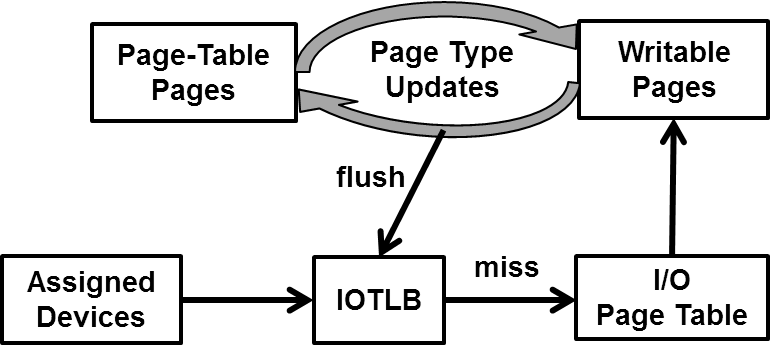
\includegraphics[width=0.5\textwidth]{image/background/problem-illustration.png} \\
\caption{DMA access has to walk along the I/O Page-Table path, which is much slower than the IOTLB path due to the frequent page type updates between writable pages and page-table pages.}
\label{fig:pro-ill}
\end{figure}

